\newpage
\section{\label{cfpmod}cfpmod}

\subsection{General}

Based on the same algorithm as used in the program {\bf extrap}, {\bf cfpmod} calculates pulse responses of sources which are defined in the subsurface. This program is therefore very usefull for the generation of CFP operators. 
\subsection{Parameters}

Via the command-line or in a parameter file: {\tt par=$<$parameter\_file$>$}.

{\footnotesize
\begin{verbatim}
  
 cfpmod - modeling one-way travel times in x-w domain
 
 cfpmod file_vel= xsrc1= zsrc1= [optional parameters]
  
 Required parameters:
 
   file_vel= ................ gridded velocity file
   xsrc1= ................... x-position of the source (m)
   zsrc1= ................... z-position of the source (m)
  
 Optional parameters:
  
   file_out= ................ output file with traveltimes
   file_int= ................ input file describing the interfaces (makemod)
   mode=1 ................... type of extrapolation (1=forward, -1=inverse)
   ntap=0 ................... number of taper points at boundaries
   n2max=512 ................ maximum number of traces in input file
   n1max=1024 ............... maximum number of samples/trace in input file
 SOURCE POSITIONS 
   xsrc2=xsrc1 .............. x-position of last source
   dxsrc=0 .................. step in source x-direction
   zsrc2=zsrc1 .............. z-position of last source
   dzsrc=0 .................. step in source z-direction
   boundary=0 ............... boundary to place the sources (overrules zsrc)
 RECEIVER POSITIONS 
   xrcv1=ox ................. x-position of the receiver (m)
   xrcv2=ox+(nx-1)*dx ....... x-position of last receiver
   dxrcv=dx ................. step in receiver x-direction
   zrcv1=oz ................. z-position of the receiver (m)
   zrcv2=zrcv1 .............. z-position of last receiver
   dzrcv=0 .................. step in receiver z-direction
   xrcv= .................... x-position's of receivers (array)
   dxspr=0 .................. step of receiver spread in x-direction
   zrcv=0 ................... z-position of the receivers (first depth level)
   lint=1 ................... linear interpolate between the rcv points
 SAMPLING AND SOURCE DEFINITION 
   file_src=<file_name> ..... wavelet in time used (overrules dt)
   file_amp=<file_name> ..... wavelet in lateral direction 
   wnx=1 .................... number of lateral wavelet samples
   dt=0.004 ................. stepsize in time-direction 
   nt=256 ................... number of time samples
   fmin=0 ................... minimum frequency 
   fmax=70 .................. maximum frequency
   add=0 .................... 1: adds all defined sources
 PLANE WAVE AREAL SHOT RECORD DEFINITION (only calculated if Na != 0)
   amin=-65 ................. minimum angle of plane wave illumination
   amax=-amin ............... maximum angle of plane wave illumination
   Na=0 ..................... number of plane waves between amin and amax
 Note that the plane waves cannot be added together by using add=1 
 EXTRAPOLATION OPERATOR DEFINITION 
   select=4 ................. type of x-w operator
   opl=25 ................... length of the convolution operator (odd)
   alpha=65 ................. maximum angle of interest
   perc=0.15 ................ smoothness of filter edge
   weight=5e-5 .............. weight factor in WLSQ operator calculation
   fine=10 .................. fine sampling in operator table
   filter=1 ................. apply kx-w filter to desired operator
   limit=1.0002.............. maximum amplitude in best operators
   opl_min=15 ............... minimum length of convolution operator
 OUTPUT 
   beam=0 ................... 1 beams, 2 add all beams for all defined shots
   verbose=0 ................ silent option; >0 display info
  
   Options for select:
         - 0 = Truncated operator
         - 1 = Gaussian tapered operator
         - 2 = Kaiser tapered operator
         - 3 = Smoothed Phase operator
         - 4 = Weighted Least Squares operator
         - 5 = Remez exchange operator
         - 8 = Smooth Weighted Least Squares operator
         - 9 = Optimum Smooth Weighted Least Squares operator
         - 10= Optimum Weighted Least Squares operator
  
  Copyright 1997, 2008 Jan Thorbecke, (janth@xs4all.nl) 
\end{verbatim}}

\subsection{General parameter description}

The gridded subsurface ({\tt file\_vel}) which is needed in the caclulation can be made with for example the DELPHI program {\bf makemod}. {\tt file\_int} is defined by the same program. 

The source position(s) are defined by coordinates in x({\tt xsrc1, xsrc2, dxsrc}) and z ({\tt zsrc1, zsrc2, dzsrc}). If {\tt file\_int} is defined then it is also possible to use the parameter {\tt boundary} instead of the z parameters. The interface file ({\tt file\_int}) is used to place the source at the defined boundary (at the defined x position). Every source postition defines one output gather. However if {\tt add=1} the defined source postions are combined to a planar source and only one output gather is calculated.

The receiver spread is defined by coordinates in x ({\tt xrcv, dxrcv}) and z ({\tt zrcv dzrcv}). The parameters {\tt xrcv} and {\tt zrcv} are defined as arrays which interpretation depends on the parameter {\tt lint}. For example if {\tt xrcv=0,3000}, {\tt zrcv=0,0}, {\tt dxrcv=15}, {\tt dzrcv=0} and {\tt lint=1} then between the points (0,0) and (3000,0) the defined receiver positions are calculated by a linear interpolation between the two points with dx=15, which results in an receiver array of 201 receivers ranging from (0,0) to (3000,0). However, if {\tt lint=0} the receivers are only defined at the points (0,0) and (3000,0). One can also use the paremeters {\tt xrcv1, xrcv2} and {\tt zrcv1, zrcv2} to define receiver arrays.
 
Once the spread for the first shot position is defined, the parameter {\tt dxspr} define the movement of the spread for the next shot.  Choosing {\tt dxspr=0} defines a fixed spread modeling.

The parameter {\tt file\_src} defines a source wavelet, however, if this parameter is not defined a wavelet with a flat spectrum and zero phase is used in the program. 
The sources can be extended in the lateral direction by using the parameter {\tt wnx} or {\tt file\_amp}.  If there are more source positions defined (with {\tt zsrc1 $\not=$ zsrc2} and {\tt dzsrc > 0}) the output consists of a number of shot gathers. The source position in the gridded model is chosen at the nearest grid position.

Plane waves are defined by using the parameters {\tt Na}, {\tt amin} and {\tt amax}. Which define the number of plane waves and the minimum and maximum angle respectively. 

For a more detailed discussion on the different parameters which are related to the operator optimization the reader is referred to the description of the program \htmlref{{\bf opercalc}}{opercalc}.

\subsection{Examples}

To run the program a gridded velocity file has to be defined. We use the gridded velocity file (synclin\_cp.su, see Figure
\ref{model}) which can
be found in the demo directory, and a ricker wavelet (ricker.su, see Figure \ref{wave}), which can also be found in the demo directory.

In this gridded subsurface file we want to place a source at depth 1000 m, at x-position 500 and model the response at the surface.
The result is shown in Figure \ref{cfp1} and the command to generate this results is:

{\footnotesize
\begin{verbatim}
../bin/cfpmod file_vel=syncline_cp.su xsrc1=1000 zsrc1=500 ntap=30 file_src=ricker.su | suximage
\end{verbatim}}
%
\begin{figure}[hb]
  \begin{pspicture}(8,6.5)
    \put(5.0,-0.3){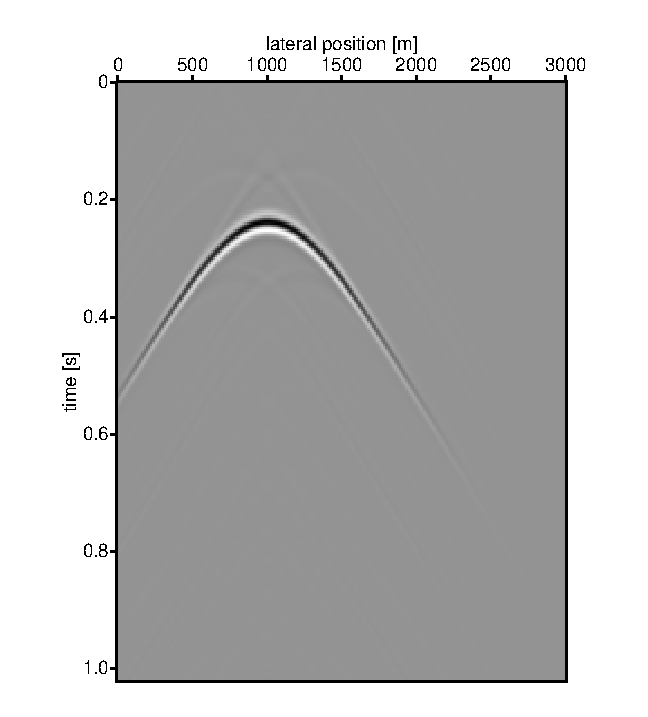
\epsfig{file=EPS/cfpmod_x1000_z500.eps,height=7cm}}
\end{pspicture}
\caption{Response of a point source at x=1000 and z=500 m., measured at the surface z=0.  } \label{cfp1}
\end{figure}
%

To calculate 5 plane wave responses, with 5 different angles ranging from -20 to 20,  from the subsurface the following command can be used:

{\footnotesize
\begin{verbatim}
../bin/cfpmod file_vel=syncline_cp.su xsrc1=1000 zsrc1=1200 ntap=30  \
    file_src=ricker.su Na=5 amin=-20 verbose=1 | suximage
\end{verbatim}}
%
\begin{figure}[hb]
  \begin{pspicture}(8,7)
    \put(-0.55,-0.3){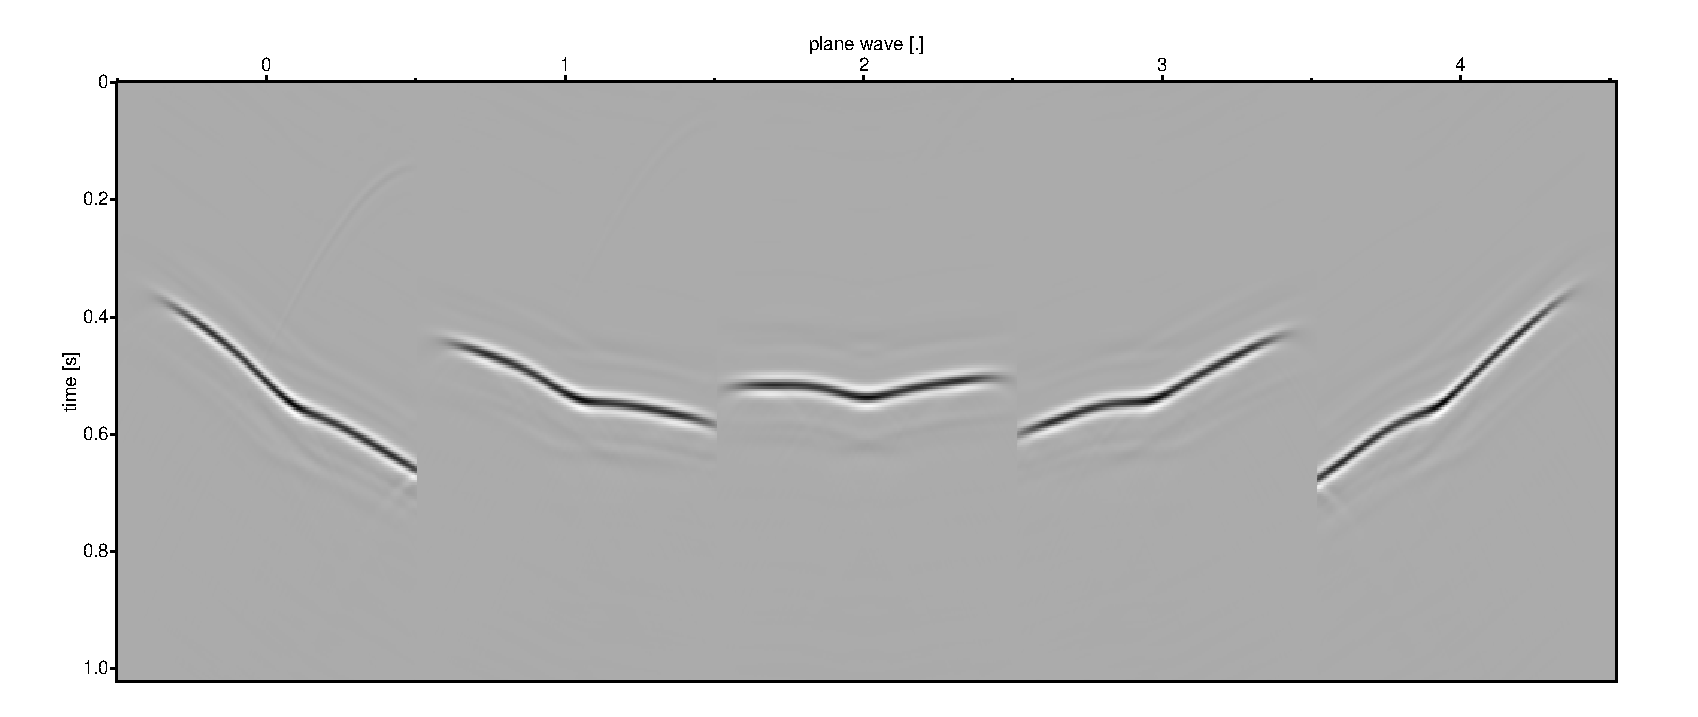
\epsfig{file=EPS/cfpmod_plane.eps,height=7cm}}
\end{pspicture}
\caption{Response of 5 plane waves at z=1200 and x=1500 with angles ranging from -20 to 20. } \label{cfp2}
\end{figure}

To model more than one source position use:

{\footnotesize
\begin{verbatim}
../bin/cfpmod file_vel=syncline_cp.su xsrc1=300 xsrc2=2700 \
    zsrc1=1200 zsrc2=1200 dxsrc=300 file_src=ricker.su \
    ntap=30 verbose=1 | suximage
\end{verbatim}}

and add those together (and do only one modeling step) do

{\footnotesize
\begin{verbatim}
../bin/cfpmod file_vel=syncline_cp.su xsrc1=300 xsrc2=2700 \
    zsrc1=1200 zsrc2=1200 dxsrc=300 file_src=ricker.su \
    ntap=30 add=1 verbose=1 | suximage
\end{verbatim}}
%
\begin{figure}[hb]
  \begin{pspicture}(8,6.5)
    \put(5.0,-0.3){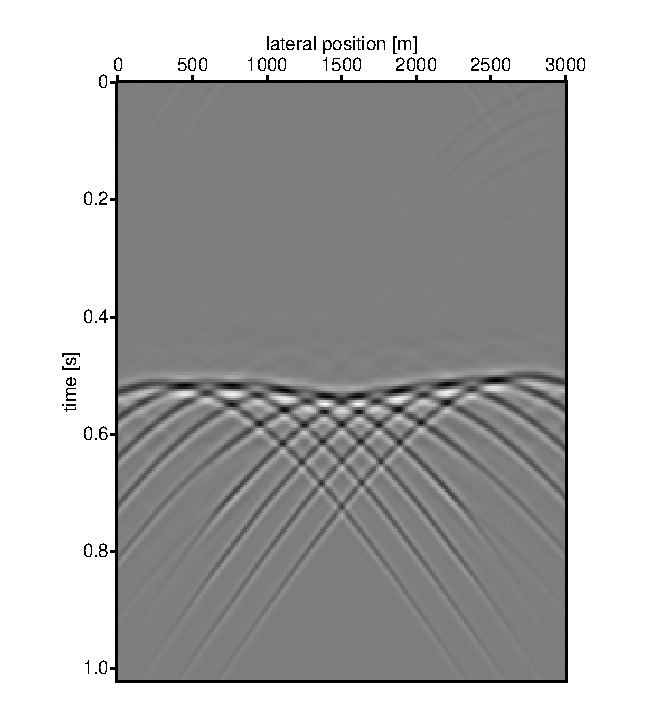
\epsfig{file=EPS/cfpmod_add.eps,height=7cm}}
\end{pspicture}
\caption{Response of several point sources position at x=[300,2700] and z=1200 m., measured at the surface z=0.  } \label{cfp3}
\end{figure}
%

\subsection{To do}
Using the local reflectivity function (or a source distribution) instead of a pulse.

Better source position definition if the source does not lie on a point defined by the subsurface grid (which is an implementation of a local extrapolation).

